\setlength{\grammarparsep}{2pt plus 1pt minus 1pt} % increase separation between rules
\setlength{\grammarindent}{12em} % increase separation between LHS/RHS
\chapter{Design}
\section{UML}
UML designs assist with the visualisation of the requirements analysis, and it demonstrates the functionality and user interactions with the system. The UML designs include the full scope of the project. The full scope includes both functional and non-functional mandatory and desirable requirements and the broader scope of the aims and objectives of the project.

\subsection{Use Case Diagram}

A use case diagram is a representation of a user's interaction with the system that shows the relationship between the user and the different use cases in which the user is involved. The use-case diagrams are split to demonstrate the users' interactions with the domain specific language and the interaction of the web-application.
\begin{figure}
  \centering
  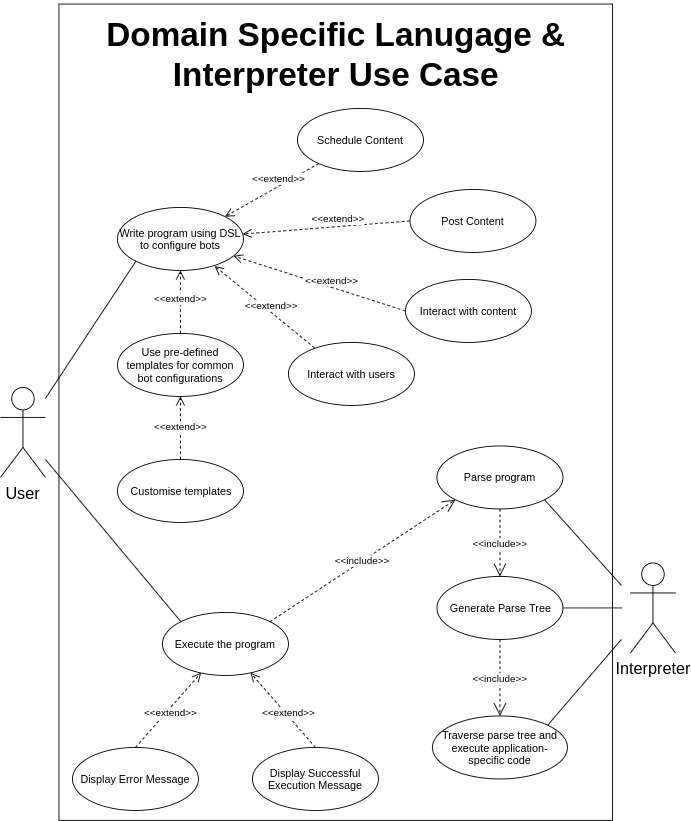
\includegraphics[width=0.9\textwidth]{images/usecasedsl.png}
  \caption{UML Use Case Diagram for DSL and Interpreter}
\end{figure}

\begin{figure}[H]
  \centering
  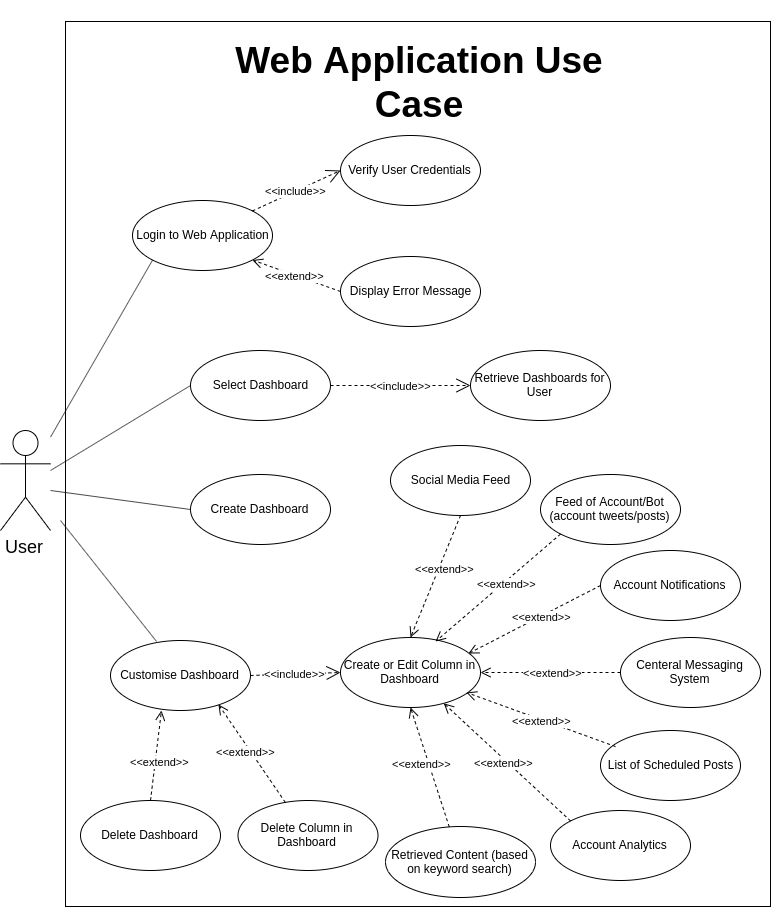
\includegraphics[width=0.9\textwidth]{images/usecasewebapp-2.png}
  \caption{UML Use Case Diagram for Web Application}
\end{figure}

\subsection{High-Level Domain Model}

The high-level domain model is a conceptual model of the domain that incorporates both behaviour and data. The domain model is a system of abstractions that describes selected aspects of a sphere of knowledge, influence or activity. The high-level domain model in figure 5.3 represents how the user interacts with the system and how the different components of the system are incorporated and interact with each other.

\begin{figure}[H]
  \centering
  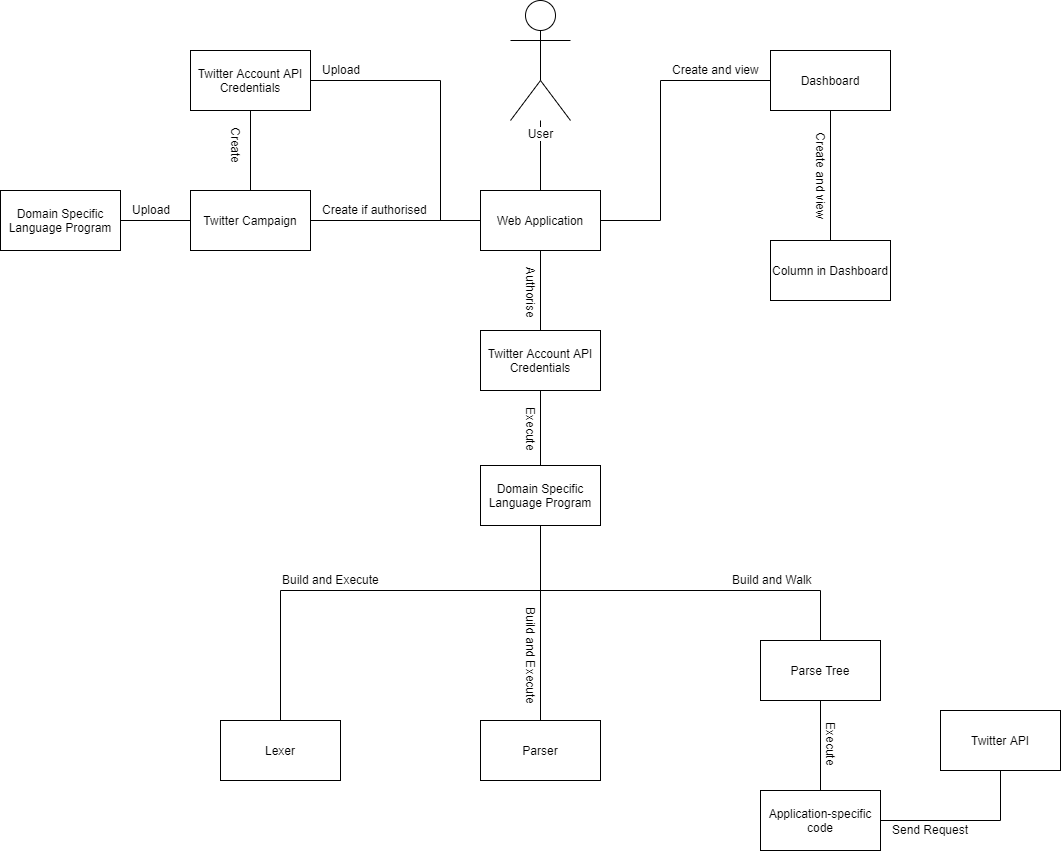
\includegraphics[width=1\textwidth]{images/high-level-domain.png}
  \caption{High-Level Domain Model}
\end{figure}

\subsection{Software Patterns}

The outcome of the high-level domain model loosely represents a conventional model-view-controller architecture. The model-view-controller architecture bases itself on three components, the model, the view and the controller. The model is the central component which usually reflects real-world objects and is used to store raw data. The view is a representation of the model to the user. The controller acts as a liaison between the model and the view and accepts user input, updates the model and produces an output for the view \cite{deacon2009model}. 

\begin{figure}[H]
  \centering
  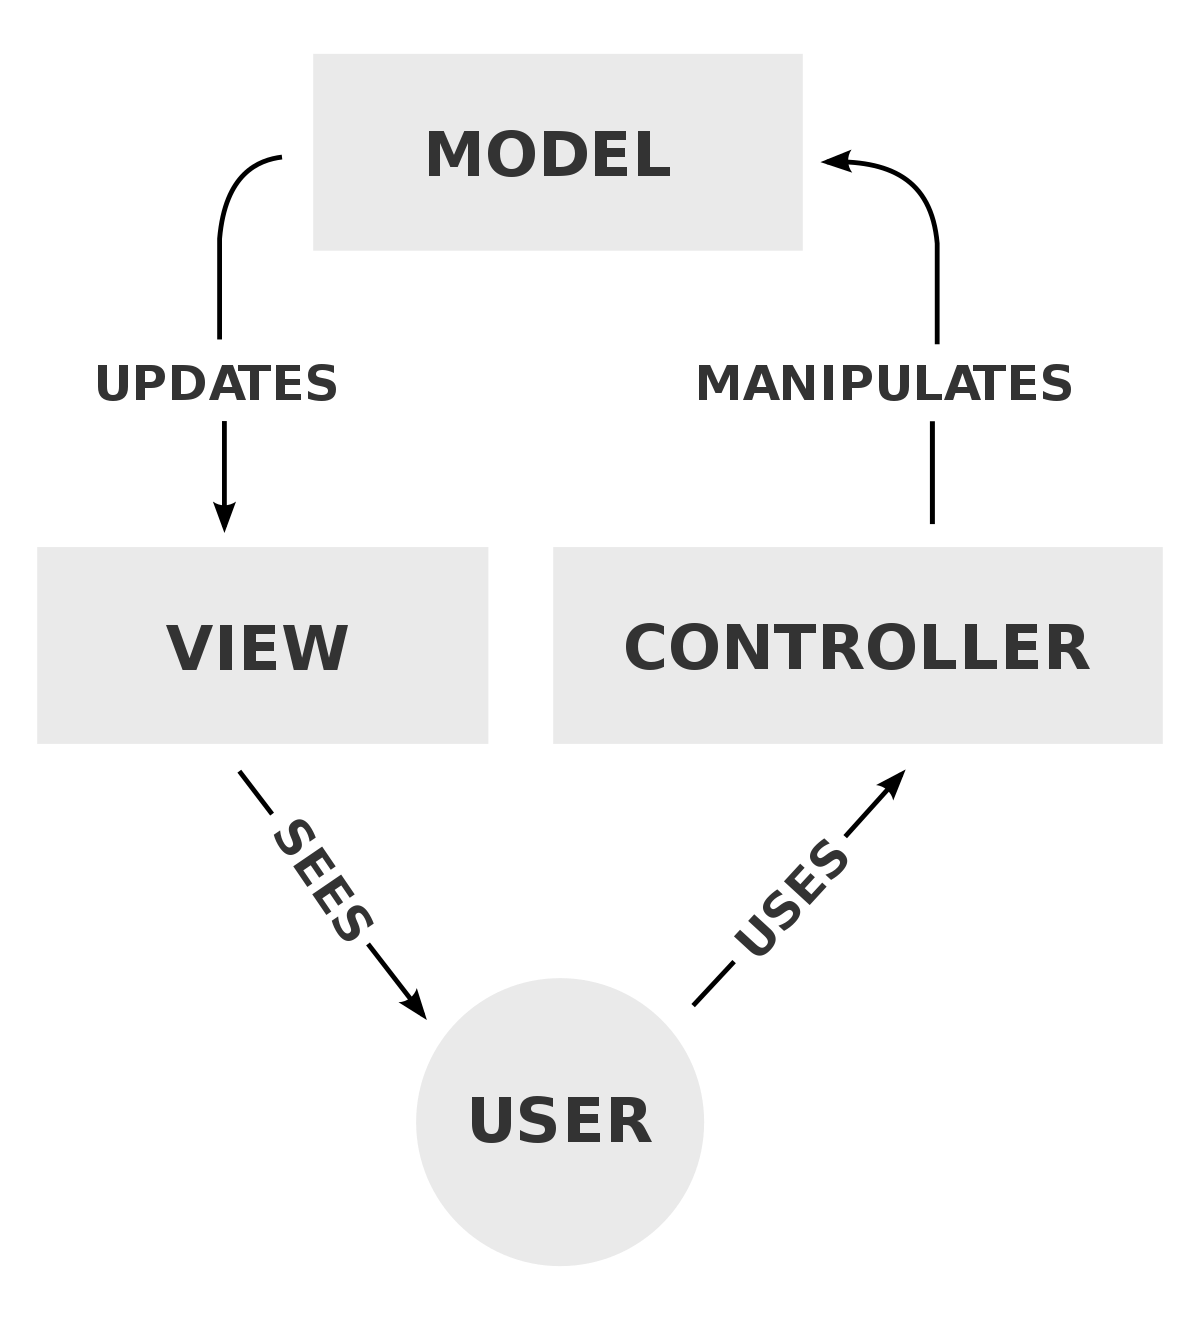
\includegraphics[width=0.3\textwidth]{images/mvc.png}
  \caption{MVC Design Pattern \cite{mvc}}
\end{figure}

A model is the single, definitive source of information about the data. It contains the required fields and behaviours of the stored data and generally, each model maps to a single database table. The model component in the high-level domain diagram represents the Twitter Account API credentials and Twitter Campaigns. The Twitter Account API credentials model stores information about the Twitter Account with API access, including the username and the consumer keys and access tokens. The Twitter Campaign model includes a name, a description, and the file to be executed. The view component in the high-level domain model represents the dashboard and the column in the dashboard to display information about the models. The domain specific language acts as the controller, which the user interacts with to manipulate the model to update the view. A potential feature of the project utilising the model-view-controller architecture is scheduling, where the user creates a scheduled post through the domain specific language, which creates a scheduled post in the model which displays in the view.

\section{Grammar}

The grammar designs define the syntactical structure of the domain specific language. Designing the grammar is the initial step for understanding the structure of a program for the domain specific language and how it will interact with the Twitter API. The first step to achieve this is to write out all the actions that the domain specific language should achieve based on the requirements analysis. The domain specific language should provide the functionality to tweet, retweet, favourite, schedule and direct message and this can be translated directly into a grammar rule `action'. \newline \par

The interaction of the Twitter API requires a RESTful service using JSON objects. An intuitive design approach for the domain specific language is to create a language with actions that generate JSON templates and values which populate the JSON object. An initial grammar design is inspired by and replicates a similar grammatical structure to JSON objects, where each action has a parameter with a key-value pair. The first grammar design, presented in extended Backus–Naur form (EBNF):

\begin{grammar}
<twitbot> ::= <statement `;'>+

<statement> ::= <action> <parameter> `,' <parameter>*

<action> ::= `tweet' 
\alt `retweet'
\alt `favourite'
\alt `schedule'
\alt `direct-message'

<parameter> ::= <identifier> `:' <value>

<identifier> ::= <string>

<value> ::= <string>

<string> ::= [a-zA-Z0-9]+
\end{grammar}

The initial grammar design is an extremely lightweight grammar as it has vasts amount of flexibility and is error-prone. This initial design of the grammar has limited and restricted functionality and power. The grammar does not include any conditional statements, types, looping or recursion. \newline \par

The first grammar does not directly represent an interaction with the Twitter API. The grammar is designed to populate JSON objects and does not provide any functionality for automation. The next design decisions evaluate the trade-offs of implementing this functionality through back-end software or extending the language further to include new features. This decision is prevalent while dealing with user authentication. For each Twitter API call a user must be authenticated. This authentication requires the user access tokens and consumer keys to be included in each Twitter API call. The current grammar design uses actions which represents a Twitter API call, and this requires each action grammar rule to include access tokens and consumer keys. A solution to this problem is to define macros in the language to retrieve user login credentials from a separate file to abstract the authentication from the user and increase code-reuse. Another solution to this is to utilise back-end software to manage the user authentication and abstract this from the user. As the requirements specify that it is mandatory for the domain specific language to be used by both programmers and non-programmers, utilising the power of back-end software keeps the language concise without adding any complexity. As the requirements analysis and the overall aims and objectives of the project are to include a web-application, the web-application will handle the management of authentication keys and tokens. \newline \par

The initial grammar lacks the majority of functionality specified in the requirements analysis, and its syntactical structure does not closely align with the problem domain. The next stage for grammar designs is to extend the actions further, splitting each action to have required and optional parameters, with the key-value pairs of these parameters encapsulating the logic of a Twitter API call. A program for the domain specific language should reflect a Twitter campaign, which allows for a list of actions to be performed and automated bot actions. An example of a Twitter Campaign for a brand is to market a new product. The program must reflect the logic of the different elements that go into a marketing campaign. This logic includes the scheduling of tweets, tweeting with images, retweeting and responding to mentions based on keywords. This leads to the final grammar design, which encapsulates the logic of having multiple tailored actions to perform different tasks. The final grammar design is presented in extended Backus–Naur form (EBNF) in appendix A.